\documentclass[11pt,a4paper]{report}

\usepackage[a4paper, margin=1in]{geometry}
\usepackage{polski}
\usepackage[utf8]{inputenc}
\usepackage{indentfirst}
\usepackage{hyperref}
\usepackage{graphicx}

\graphicspath{ {./images/} }

\def\console #1{\begingroup\fontfamily{qcr}\selectfont#1\endgroup}
\newenvironment{multiconsole}{\begingroup\fontfamily{qcr}\selectfont}{\endgroup}



\title{\Huge JavaGridGraph - Sprawozdanie}
\author{Skoczek Mateusz, Jędrzejewski Sebastian}
\date{\today}



\begin{document}
    \maketitle
        




    \begin{abstract}
        Dokument zawiera specyfikację funkcjonalną i implementacyjną dotyczącą projektu \textsl{JavaGridGraph} oraz opis testów programu.
    \end{abstract}





    \tableofcontents
    \thispagestyle{empty}





    \newpage
    \chapter{Specyfikacja funkcjonalna}




    \newpage
    \section{Cel projektu}

    Program \textbf{JavaGridGraph} ma na celu umożliwiać wykonanie dwóch podstawowych zadań

    \begin{itemize}
        \item wygenerowanie grafu siatkowego o podanych paramentrach
        \item sprawdzenie wybranych parametrów dowolnego grafu siatkowego
    \end{itemize}

    Program posiada interfejs graficzny. Grafy są przedstawiane w plikach w postaci listy sąsiedztwa.




    \newpage
    \section{Opis funkcji}

    Program oferuje dwie główne funkcje: generowanie grafu oraz sprawdzanie grafu.

    \vspace{4em}

    Program pozwala wygenerować graf o:
    
    \begin{itemize}
        \item określonej wysokości (ilości wierszy)
        \item określonej szerokości (ilości kolumn)
        \item określonej minimalnej i maksymalnej wadze krawędzi
        \item określonej minimalnej i maksymalnej ilości krawędzi wychodzących z pojedyńczego wierzchołka (dla grafu skierowanego)
        \item określonej minimalnej i maksymalnej ilości krawędzi wchodzących do pojedyńczego wierzchołka (dla grafu skierowanego)
        \item określonej minimalnej i maksymalnej ilości "sąsiadów" pojedyńczego wierzchołka (dla grafu nieskierowanego)
        \item niestandardowym ziarnie generatora liczb losowych
    \end{itemize}

    Program umożliwia zapis wygenerowanego grafu do pliku oraz/lub wczytanie grafu do sprawdzenia.
    
    \vspace{4em}

    W ramach funkcji sprawdzania grafu, program pozwala na sprawdzenie następujących parametrów wczytanego grafu:

    \begin{itemize}
        \item spójność grafu
        \item najkrótsze ścieżki od wybranego wierzchołka $A$ do wybranych wierzchołków $B_n$
    \end{itemize}




    \newpage
    \section{Opis interfejsu programu}

    \subsection{Okno główne - widok startowy}

    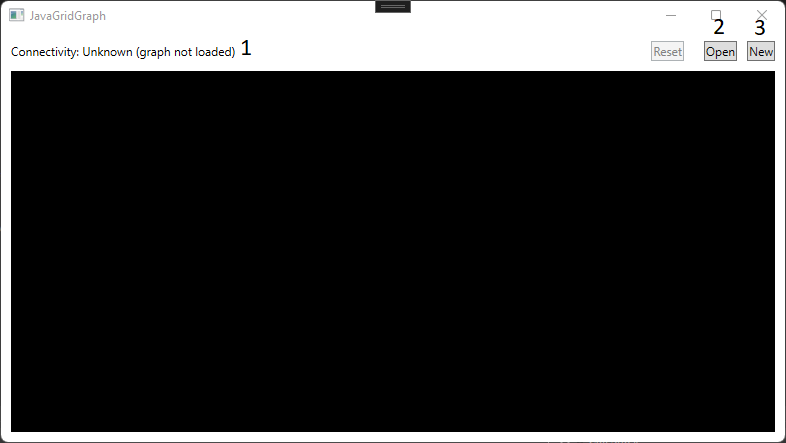
\includegraphics[width=\textwidth]{view1.png}

    \begin{enumerate}
        \item Wynik sprawdzenia spójności grafu. W przypadku gdy graf nie został wczytany, zostanie pokazana informacja o tym że graf nie został wczytany.
        \item Przycisk "Open" otwiera systemowe okno wyboru pliku w celu wybrania pliku zawierającego graf.
        \item Przycisk "New" otwiera okno generowania grafu. Więcej informacji w punkcie "Okno generowania grafu".
    \end{enumerate}

    \subsection{Okno generowania grafu}

    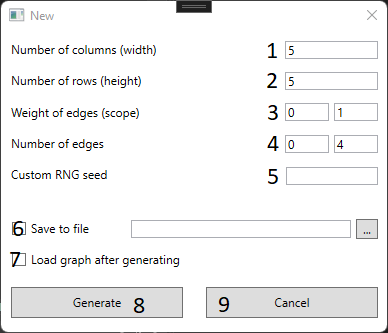
\includegraphics[width=\textwidth]{view2.png}

    \begin{enumerate}
        \item Liczba kolumn (szerokość) grafu. Pole nie może być puste.
        \item Liczba wierszy (wysokość) grafu. Pole nie może być puste.
        \item Waga krawędzi. Wartość w pierwszym polu (min, domyślnie 0) musi być mniejsza bądź równa wartości w drugim polu (max, domyślnie 1).
        \item Wybór między generowaniem grafu skierowanego (directed), generowaniem grafu nieskierowanego (not directed).
        \item Liczba krawędzi wychodzących z pojedyńczego wierzchołka. Wartość w pierwszym polu (min, domyślnie 0) musi być mniejsza bądź równa wartości w drugim polu (max, domyślnie 4). [Tylko gdy zaznaczone generowanie grafu skierowanego]\footnote{Program będzie dążył do utworzenia co najmniej minimalnej liczby krawędzi (połączeń do sąsiadów), ale nie może tego zagwarantować. Nie jest możliwe wygenerowanie więcej niż 2 krawędzi dla wierzchołków w narożnikach oraz więcej niż 3 dla wierzchołków bocznych. Nie jest możliwe także utworzenie krawędzi, jeżeli wszystkie wierzchołki wokół osiągnęły już swoją nominalną (wylosowaną z podanego przedziału) liczbę krawędzi.}
        \item Liczba krawędzi wchodzących do pojedyńczego wierzchołka. Wartość w pierwszym polu (min, domyślnie 0) musi być mniejsza bądź równa wartości w drugim polu (max, domyślnie 4). [Tylko gdy zaznaczone generowanie grafu skierowanego]\footnotemark[\value{footnote}]
        \item Liczba sąsiadów pojedyńczego wierzchołka. Wartość w pierwszym polu (min, domyślnie 0) musi być mniejsza bądź równa wartości w drugim polu (max, domyślnie 4). [Tylko gdy zaznaczone generowanie grafu nieskierowanego]\footnotemark[\value{footnote}]
        \item Niestandardowe ziarno generatora liczb losowych.
        \item Zaznaczenie tego pola spowoduje zapisanie grafu w pliku wybranym w systemowym oknie zapisu pliku, które wyświetli się po naciśnięciu przycisku "Generate".
        \item Zaznaczenie tego pola spowoduje wczytanie grafu do programu zaraz po jego wygenerowaniu.
        \item Kliknięcie przycisku spowoduje wygenerowanie grafu o podanych parametrach.
    \end{enumerate}

    \subsection{Okno główne - po wczytaniu grafu}

    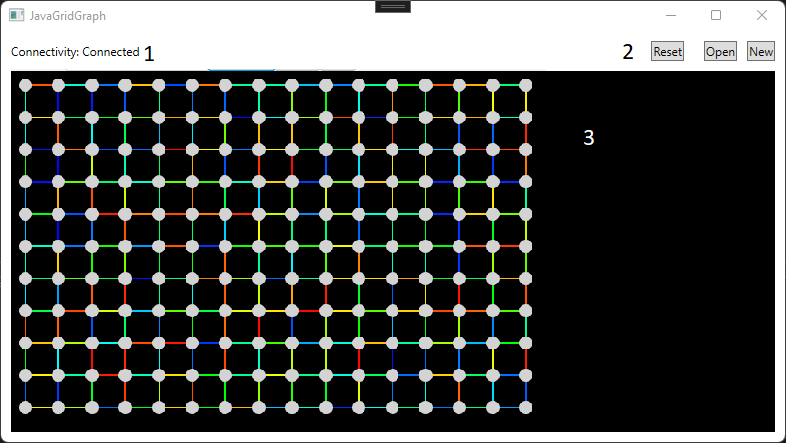
\includegraphics[width=\textwidth]{view3.png}

    \begin{enumerate}
        \item Wynik sprawdzenia spójności grafu. "Connected" - spójny, "Unconnected" - niespójny.
        \item Kliknięcie przycisku spowoduje odznaczenie wszystkich zaznaczonych wierzchołków na grafie.
        \item Pole w którym wyświetlany jest graf. Aby znaleźć najkrótsze ścieżki musimy wybrać wierzchołek $A$ lewym przyciskiem myszy (zostanie zaznaczony na czerwono) oraz wierzchołki $B_n$ prawym przyciskiem myszy (zostaną zaznaczone na zielono). Po wybraniu wierzchołka $A$ oraz przynajmniej jednego wierzchołka $B$ zostanie narysowana najkrótsza ścieżka od wierzchołka $A$ do wierzchołka $B_n$.
    \end{enumerate}




    \newpage
    \section{Format danych wejściowych i wyjściowych}
    Dane wejściowe i wyjściowe przechowują graf w postaci listy sąsiedztwa. W pierwszej linijce znajdują się dwie liczby, które oznaczają odpowiednio liczbę kolumn i wierszy danego grafu. Każda następna linijka reprezentuje jeden wierzchołek, przy czym wierzchołki numerujemy od 0 od lewej do prawej. Zatem druga linijka w pliku zawiera numery wierzchołków, z którymi połączony jest wierzchołek numer 0, kolejna dotyczy wierzchołka numer 1 itd. Przy każdym numerze wierzchołka po dwukropku podana jest waga krawędzi pomiędzy tymi dwoma wierzchołkami.

    \vspace{1em}

    \noindent
    \textbf{Przykład:}

    \begin{multiconsole}
        2 2

        \hspace*{2em}1 :0.54  2 :0.78

        \hspace*{2em}0 :0.54  3 :0.12

        \hspace*{2em}0 :0.78  3 :0.89

        \hspace*{2em}1 :0.12  2 :0.89
    \end{multiconsole}

    Powyżej przedstawiona jest przykładowa zawartość pliku przechowującego graf. W pierwszej linijce można odczytać, że jest to graf o dwóch kolumnach i dwóch wierszach. W drugiej linijce przedstawiona jest informacja o tym, że wierzchołek numer 0 połączony jest z wierzchołkiem numer 1, a krawędź ta ma wagę 0.54. Istnieje również krawędź pomiędzy wierzchołkiem 0 a 2 o wadze 0.78. W trzeciej linijce znajdują się numery wierzchołków połączonych z wierzchołkiem numer 1 wraz z wagami itd.





    \newpage
    \chapter{Specyfikacja implementacyjna}




    \newpage
    \section{Diagram klas}
    \begin{center}
        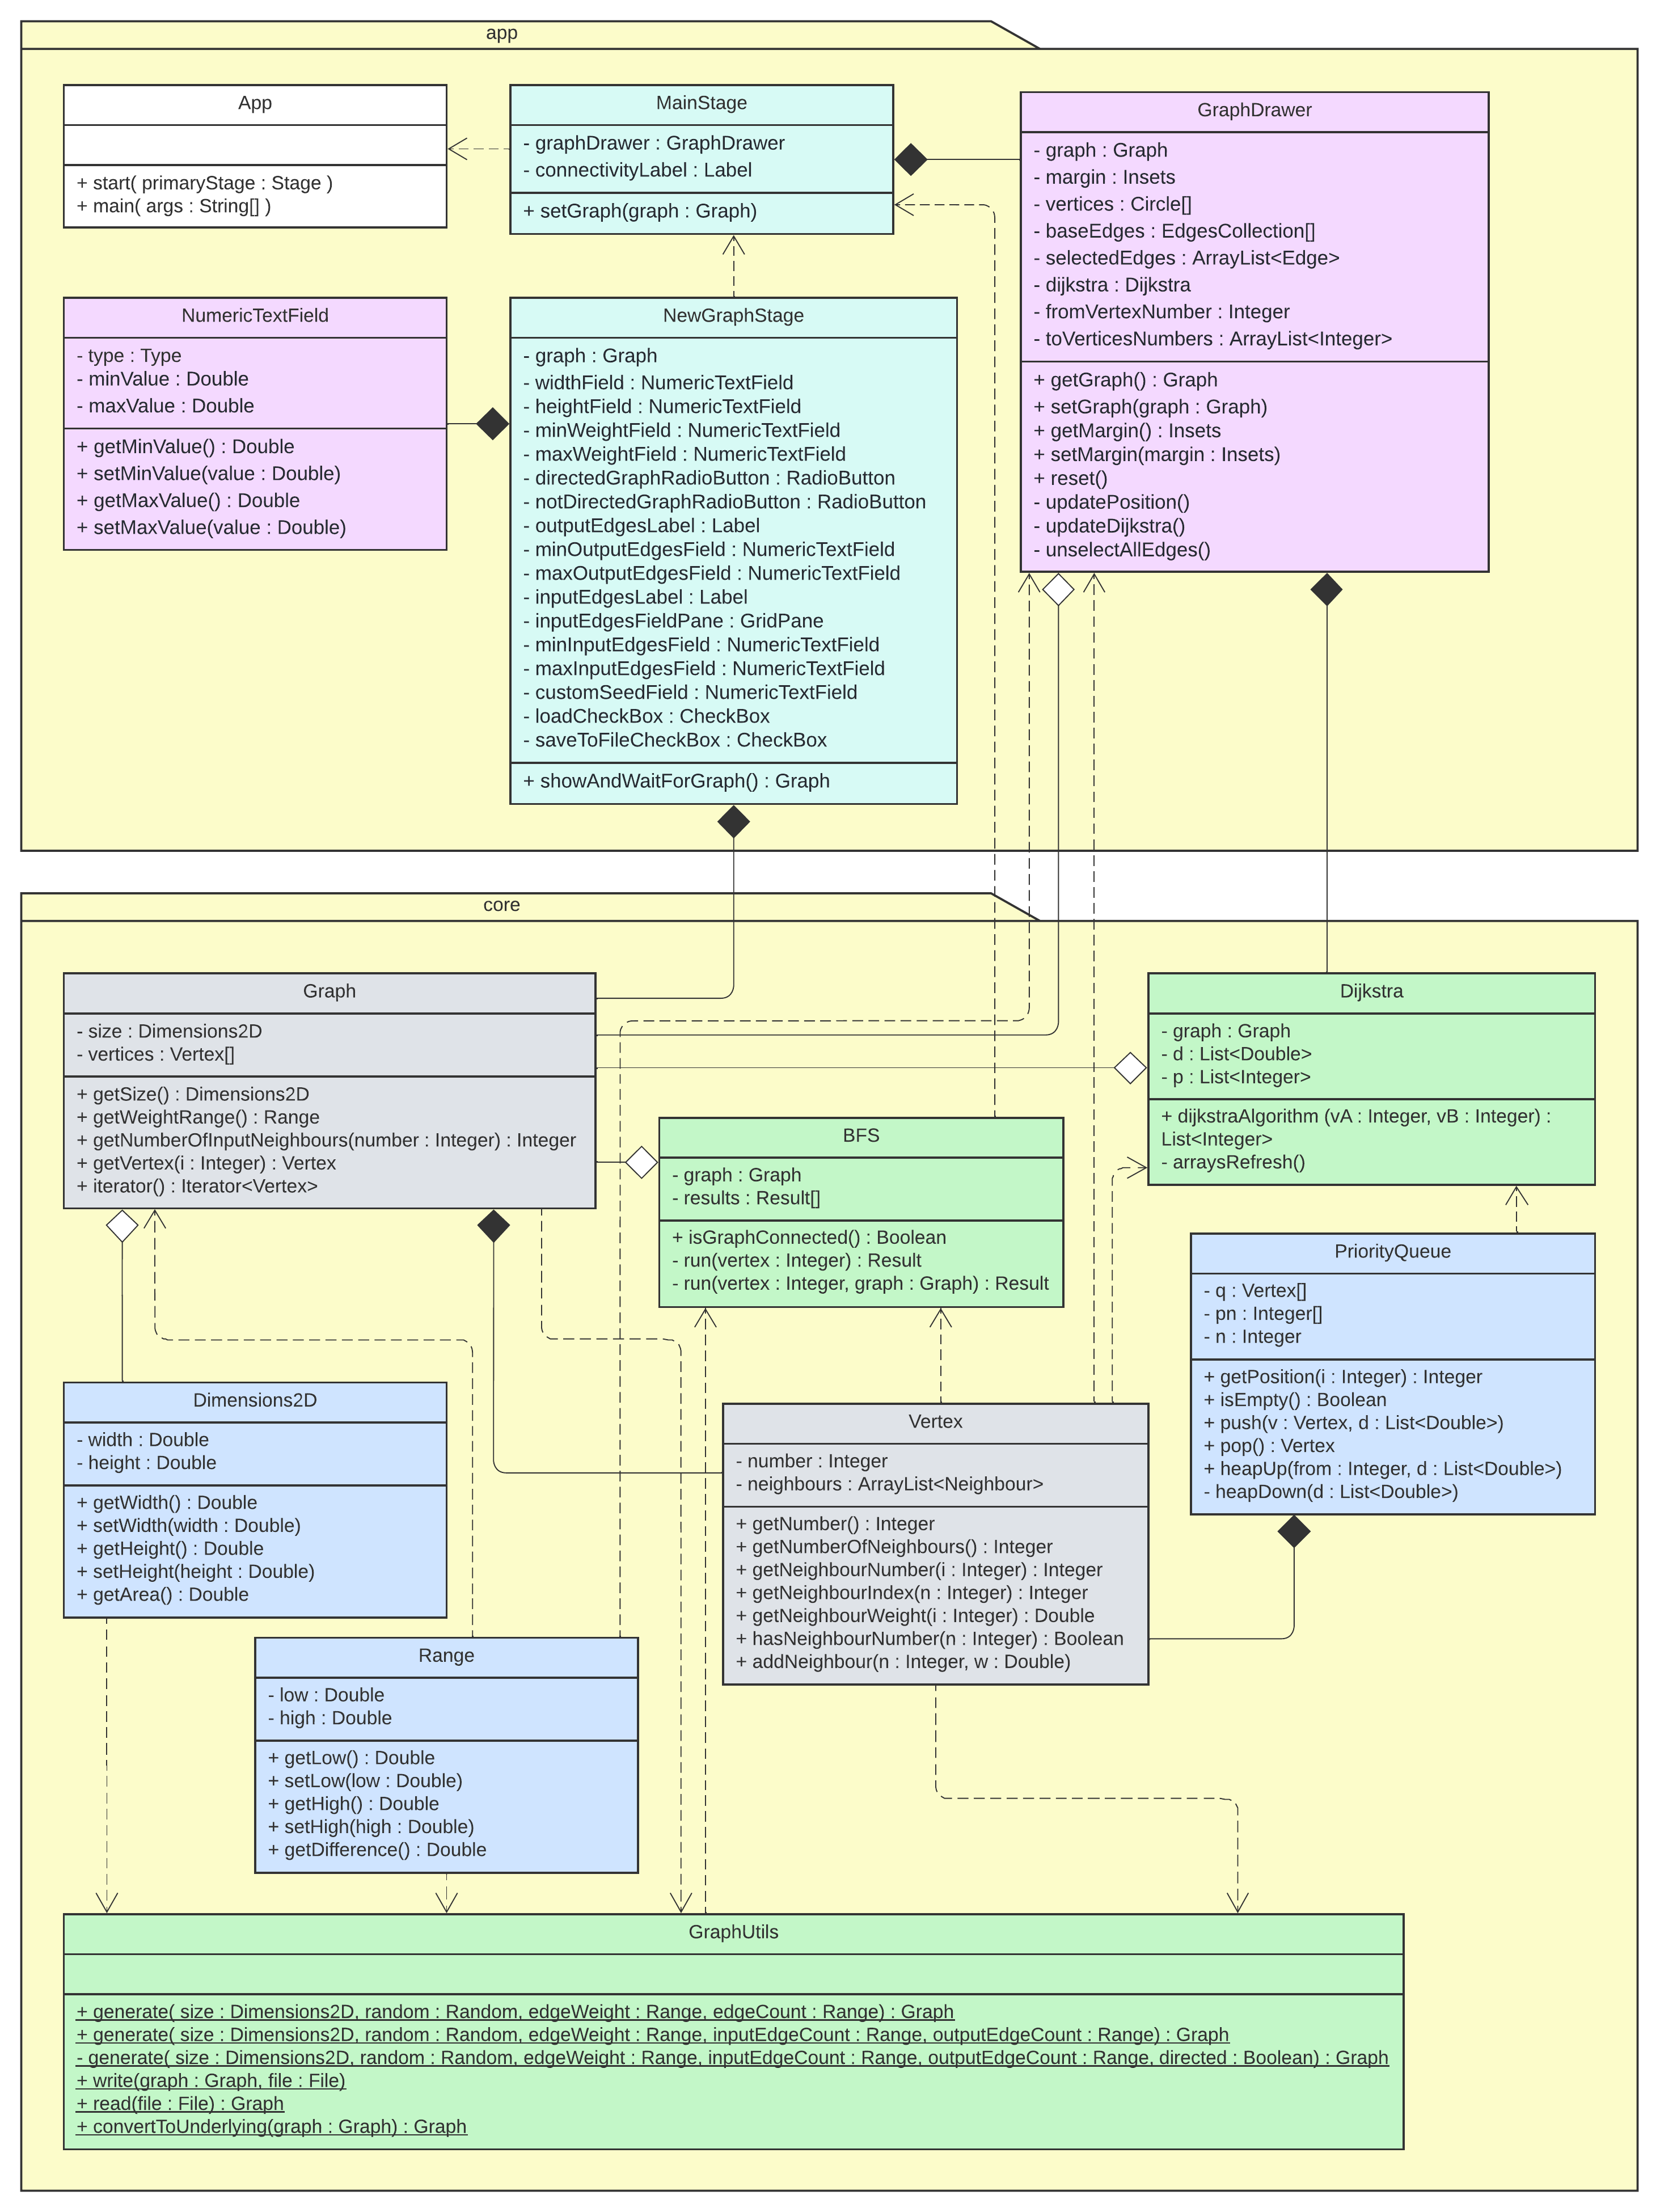
\includegraphics[width=\textwidth]{uml.png}
    \end{center}



    \newpage
    \section{Pakiet App (Interfejs)}

    Interfejs aplikacji został stworzony przy wykorzystaniu biblioteki JavaFX. Pakiet \textbf{App} składa się z dwóch podpakietów:

    \begin{itemize}
        \item \textbf{Stages} zawierającym widoki aplikacji
        \item \textbf{Controls} zawierającym niestandardowe kontrolki
    \end{itemize}

    \vspace{3em}


    \subsection{App (App)}

    Klasa App jest główną klasą całej aplikacji. Dziedziczy ona po klasie \console{Application} należącej do pakietu \console{javafx.application}

    \vspace{2em}

    \textbf{Publiczne metody:}

    \begin{itemize}
        \item \console{public void start(Stage primaryStage)} - Odpowiada za utworzenie głównego okna aplikacji (\console{MainStage}) i pokazanie go.
        \item \console{public static void main(String[] args)} - Jest entry pointem i odpowiada za zainicjowanie aplikacji.
    \end{itemize}

    \vspace{2em}


    \subsection{MainStage (App.Stages)}

    Klasa MainStage jest odpowiedzialna za główne okno aplikacji. Dziedziczy ona po klasie \console{Stage} należącej do pakietu \console{javafx.stage}

    \vspace{2em}

    \textbf{Właściwości:}

    \begin{itemize}
        \item \console{private final GraphDrawer graphDrawer}
        \item \console{private final Label connectivityLabel}
    \end{itemize}

    \vspace{2em}

    \textbf{Konstruktory:}

    \begin{itemize}
        \item \console{public MainStage()} - Główny konstruktor. W konstruktorze inicjowane jest okno (tworzone są kontrolki) i ustawiane są właściwości okna.
    \end{itemize}

    \vspace{2em}

    \textbf{Publiczne metody:}

    \begin{itemize}
        \item \console{public void setGraph(Graph graph)} - Metoda odpowiedzialna za ustawienie grafu w kontrolce \console{graphDrawer} oraz sprawdzenie i wyświetlenie infromacji (w kontrolce \console{connectivityLabel}) o spójności grafu.
    \end{itemize}

    \vspace{2em}

    \textbf{Obsługa zdarzeń:}

    \begin{itemize}
        \item \console{LoadGraphButtonClicked} - Obsługuje zdarzenie naciśnięcia przycisku ładowania grafu z pliku. Otwiera systemowe okno otwierania pliku. Po wybraniu pliku wywoływana jest metoda \console{setGraph}.
        \item \console{ResetGraphDrawerButtonClicked} - Obsługuje zdarzenie naciśnięcia przycisku resetowania kontrolki wyświetlającej graf. Czyści zaznaczone ścieżki i wierzchołki (wywołuje metodę \console{graphDrawer.reset()}).
        \item \console{NewGraphButtonClicked} - Obsługuje zdarzenie naciśnięcia przycisku tworzenia nowego grafu. Tworzy okno tworzenia grafu \console{NewGraphStage}, wyświetla je oraz wywołuje metodę \console{setGraph} dla zwróconego grafu.
    \end{itemize}

    \vspace{2em}


    \subsection{NewGraphStage (App.Stages)}

    Klasa NewGraphStage jest odpowiedzialna za okno tworzenia grafu. Dziedziczy ona po klasie \console{Stage} należącej do pakietu \console{javafx.stage}

    \vspace{2em}

    \textbf{Właściwości:}

    \begin{itemize}
        \item \console{private Graph graph} - Graf który zostanie zwrócony w przypadku zamknięcia okna.
        \item \console{private final NumericTextField widthField}
        \item \console{private final NumericTextField heightField}
        \item \console{private final NumericTextField minWeightField}
        \item \console{private final NumericTextField maxWeightField}
        \item \console{private final RadioButton directedGraphRadioButton}
        \item \console{private final RadioButton notDirectedGraphRadioButton}
        \item \console{private final Label outputEdgesLabel}
        \item \console{private final NumericTextField minOutputEdgesField}
        \item \console{private final NumericTextField maxOutputEdgesField}
        \item \console{private final Label inputEdgesLabel}
        \item \console{private final GridPane inputEdgesFieldPane}
        \item \console{private final NumericTextField minInputEdgesField}
        \item \console{private final NumericTextField maxInputEdgesField}
        \item \console{private final NumericTextField customSeedField}
        \item \console{private final CheckBox loadCheckBox}
        \item \console{private final CheckBox saveToFileCheckBox}
    \end{itemize}

    \vspace{2em}

    \textbf{Konstruktory:}

    \begin{itemize}
        \item \console{public NewGraphStage()} - Główny konstruktor. W konstruktorze inicjowane jest okno (tworzone są kontrolki) i ustawiane są właściwości okna.
    \end{itemize}

    \vspace{2em}

    \textbf{Publiczne metody:}

    \begin{itemize}
        \item \console{public Graph showAndWaitForGraph()} - Metoda odpowiedzialna za wyświetlenie okna, a po jego zamknięciu - zwrócenie grafu.
    \end{itemize}

    \vspace{2em}

    \textbf{Obsługa zdarzeń:}

    \begin{itemize}
        \item \console{GenerateButtonClicked} - Obsługuje zdarzenie naciśnięcia przycisku generowania grafu. Sprawdza podane parametry grafu, a następnie generuje graf. W przypadku gdy została wybrana opcja zapisu grafu w pliku (\console{saveToFileCheckBox}), otwiera systemowe okno zapisu pliku i zapisuje w nim wygenerowany graf. Na koniec zamyka okno.
        \item \console{DirectedGraphRadioButtonToggleGroupToggleChanged} - Obsługuje zdarzenie zmiany zaznaczenia przycisków (RadioButton) "Directed" (\console{directedGraphRadioButton}) i "Not directed" (\console{notDirectedGraphRadioButton}).
    \end{itemize}

    \vspace{2em}


    \subsection{GraphDrawer (App.Controls)}

    Klasa GraphDrawer jest odpowiedzialna za kontrolkę wyświetlającą graf. Dziedziczy ona po klasie \console{AnchorPane} należącej do pakietu \console{javafx.scene.layout}

    \vspace{2em}

    \textbf{Właściwości:}

    \begin{itemize}
        \item \console{private Graph graph} - Aktualnie ustawiony w kontrolce graf
        \item \console{private Insets margin} - Margines kontrolki
        \item \console{private Circle[] vertices} - Tablica zawierająca reprezentację wierzchołków
        \item \console{private EdgesCollection[] baseEdges} - Tablica zawierająca kolekcję krawędzi wychodzących z wierzchołka o indeksie odpowiadającym indeksowi w tablicy
        \item \console{private ArrayList<Edge> selectedEdges} - Lista zawierająca zaznaczone krawędzie.
        \item \console{private Dijkstra dijkstra} - Algorytm Dijkstra dla aktualnie ustawionego grafu.
        \item \console{private int fromVertexNumber} - Aktualnie zaznaczony wierzchołek "od" (zaznaczony na grafie kolorem czerwonym)
        \item \console{private ArrayList<Integer> toVerticesNumbers} - Lista aktualnie zaznaczonych wierzchołków "do" (zaznaczone na grafie kolorem zielonym)
    \end{itemize}

    \vspace{2em}

    \textbf{Konstruktory:}

    \begin{itemize}
        \item \console{public GraphDrawer()} - Główny konstruktor. W konstruktorze ustawiane są domyślne własciwości kontrolki.
    \end{itemize}

    \vspace{2em}

    \textbf{Publiczne metody:}

    \begin{itemize}
        \item \console{public Graph getGraph()} - Metoda zwraca aktualnie ustawiony graf
        \item \console{public void setGraph(Graph graph)} - Metoda ustawia podany graf w kontrolce.
        \item \console{public Insets getMargin()} - Metoda zwraca margines kontrolki 
        \item \console{public void setMargin(Insets margin)} - Metoda ustawia podany margine kontrolki.
        \item \console{public void reset()} - Metoda czyści zaznaczenia wierzchołków i ścieżek
    \end{itemize}

    \vspace{2em}

    \textbf{Prywatne metody:}

    \begin{itemize}
        \item \console{public void updatePosition()} - Metoda uaktualnia pozycje wierzchołków i krawędzi.
        \item \console{public void updateDijkstra()} - Metoda uaktualnia zaznaczone krawędzie
        \item \console{public void unselectAllEdges()} - Metoda usuwa zaznaczenia ze wszystkich krawędzi.
    \end{itemize}

    \vspace{2em}

    \textbf{Klasy zagnieżdzone:}

    \begin{itemize}
        \item \console{private class EdgesCollection} - Przechowuje reprezentacje krawędzi wychodzących z pojedyńćzego wierzchołka we wszystkich kierunkach.
        \item \console{private class Edge extends Group} - Zespół kontrolek Circle i Line, będących reprezentacją krawędzi. Dziedziczy po klasie \console{Group} należącej do pakietu \console{javafx.scene}
    \end{itemize}

    \vspace{2em}


    \subsection{NumericTextField (App.Controls)}

    Klasa NumericTextField jest modyfikacją kontrolki \console{TextField} pozwalającą na wpisywanie tylko liczb. Dziedziczy ona po klasie \console{TextField} należącej do pakietu \console{javafx.scene.control}

    \vspace{2em}

    \textbf{Właściwości:}

    \begin{itemize}
        \item \console{private final Type type} - Typ liczb wpisywanych w pole.
        \item \console{private double minValue} - Dolny zakres liczb wpisywanych w pole.
        \item \console{private double maxValue} - Górny zakres liczb wpisywanych w pole.
    \end{itemize}

    \vspace{2em}

    \textbf{Konstruktory:}

    \begin{itemize}
        \item \console{public NumericTextField(Type type)} - Konstruktor wywołujący główny konstruktor. Jako wartość początkową w polu ustawia pusty napis.
        \item \console{public NumericTextField(Type type, String text)} - Główny konstruktor.
    \end{itemize}

    \vspace{2em}

    \textbf{Publiczne metody:}

    \begin{itemize}
        \item \console{public double getMinValue()} - Metoda zwraca dolny zakres liczb wpisywanych w pole
        \item \console{public void setMinValue(double value)} - Metoda ustawia dolny zakres liczb wpisywanych w pole
        \item \console{public double getMaxValue()} - Metoda zwraca górny zakres liczb wpisywanych w pole
        \item \console{public void setMaxValue(double value)} - Metoda ustawia górny zakres liczb wpisywanych w pole
    \end{itemize}

    \vspace{2em}

    \textbf{Obsługa zdarzeń:}

    \begin{itemize}
        \item \console{TextChanged} - Obsługuje zdarzenie zmiany tekstu w polu. Sprawdza wprowadzoną liczbę pod kątem ustawionych własciwości kontrolki.
    \end{itemize}

    \vspace{2em}

    \textbf{Wyliczenia:}

    \begin{itemize}
        \item \console{Type} - Typ wprowadzanych w kontrolce liczb
    \end{itemize}



    \newpage
    \section{Pakiet Core}

    Pakiet \textbf{Core} składa się z dwóch podpakietów:

    \begin{itemize}
        \item \textbf{GraphAlgorithms} zawierającym algorytmy grafowe
        \item \textbf{Helpers} zawierającym klasy pomocnicze.
    \end{itemize}

    \vspace{3em}


    \subsection{Graph (Core)}

    Klasa Graph jest odpowiedzialna za przechowywanie grafu siatkowego w formie listy sąsiedztwa. Implementuje ona interfejs \console{Iterable}.

    \vspace{2em}

    \textbf{Właściwości:}

    \begin{itemize}
        \item \console{private final Dimensions2D size} - Rozmiar grafu.
        \item \console{private final Vertex[] vertices} - Tablica wierzchołków.
    \end{itemize}

    \vspace{2em}

    \textbf{Konstruktory:}

    \begin{itemize}
        \item \console{public Graph(Dimensions2D size)} - Główny konstruktor.
    \end{itemize}

    \vspace{2em}

    \textbf{Publiczne metody:}

    \begin{itemize}
        \item \console{public Dimensions2D getSize()} - Metoda zwraca rozmiar grafu
        \item \console{public Range getWeightRange()} - Metoda zwraca dolną i górną granicę (najmniejszą i największą wagę) wszystkich wag krawędzi.
        \item \console{public int getNumberOfInputNeighbours(int number)} - Metoda zwraca liczbę krawędzi wchodzących do danego wierzchołka
        \item \console{public int getVertex(int i)} - Metoda zwraca wierzchołek o podanym indeksie
        \item \console{public int refresh()} - Metoda resetuje dla wszystkich wierzchołków dane wygenerowane przez algorytm Dijkstry
    \end{itemize}

    \vspace{2em}


    \subsection{Graph (Core)}

    Klasa Vertex jest odpowiedzialna za informacji o wierzchołku grafu.

    \vspace{2em}

    \textbf{Właściwości:}

    \begin{itemize}
        \item \console{private final int number} - Numer wierzchołka.
        \item \console{private double d} - Dystans od wierzchołka "od". Ustawiane przez algorytm Dijkstry.
        \item \console{private int p} - Poprzednik wierzchołka. Ustawiane przez algorytm Dijkstry.
        \item \console{private final ArrayList<Neighbour> neighbours} - Lista krawędzi wychodzących z wierzchołka (sąsiadów)
    \end{itemize}

    \vspace{2em}

    \textbf{Konstruktory:}

    \begin{itemize}
        \item \console{public Vertex(int n)} - Główny konstruktor.
    \end{itemize}

    \vspace{2em}

    \textbf{Publiczne metody:}

    \begin{itemize}
        \item \console{public int getNumber()} - Metoda zwraca numer wierzchołka
        \item \console{public double getD()} - Metoda zwraca dystans do wierzchołka "od"
        \item \console{public int getP()} - Metoda zwraca numer poprzednika wierzchołka
        \item \console{public void setD(double d)} - Metoda ustawia dystans do wierzchołka "od"
        \item \console{public void setP(int p)} - Metoda ustawia numer poprzednika wierzchołka
        \item \console{public int getNumberOfNeighbours()} - Metoda zwraca ilość krawędzi wychodzących z wierzchołka (sąsiadów)
        \item \console{public int getNeighbourNumber(int i)} - Metoda zwraca numer sąsiada w grafie, na podstawie jego indeksu w tablicy sąsiadów
        \item \console{public int getNeighbourIndex(int n)} - Metoda zwraca index sąsiada w tablicy sąsiadów, na podstawie jego numeru w grafie
        \item \console{public double getNeighbourWeight(int i)} - Metoda zwraca wagę krawędzi połączonej z sąsiadem o podanym indeksie w tablicy sąsiadów
        \item \console{public boolean hasNeighbourNumber(int n)} - Metoda zwraca wartość prawda/fałsz zapytania czy w tablcy sąsiadów znajduje się wierzchołek o podanym numerze w grafie
        \item \console{public void addNeighbour(int n, double w)} - Metoda dodaje nowego sąsiada do tablicy sąsiadów
    \end{itemize}

    \vspace{2em}

    \textbf{Klasy zagnieżdzone:}

    \begin{itemize}
        \item \console{static class Neighbour} - Przechowuje informacje (numer sąsiada i wagę) o krawędzi
    \end{itemize}

    \vspace{2em}


    \subsection{GraphUtils (Core.GraphAlgorithms)}

    Klasa GraphUtils przechowuje metody pomocnicze dla grafów

    \vspace{2em}

    \textbf{Metody:}

    \begin{itemize}
        \item \console{public static Graph generate(Dimensions2D size, Random random, Range edgeWeight, Range edgeCount)} - Metoda wywołuje główną metodę \console{generate} z opcją generowania grafu nieskierowanego
        \item \console{public static Graph generate(Dimensions2D size, Random random, Range edgeWeight, Range inputEdgeCount, Range outputEdgeCount)} - Metoda wywołuje główną metodę \console{generate} z opcją generowania grafu skierowanego
        \item \console{private static Graph generate(Dimensions2D size, Random random, Range edgeWeight, Range inputEdgeCount, Range outputEdgeCount, boolean directed)} - Metoda generuje graf o podanych parametrach
        \item \console{public static void write(Graph graph, File file)} - Metoda zapisuje graf w podanym pliku
        \item \console{public static Graph read(File file)} - Metoda czyta graf z pliku
        \item \console{public static Graph convertToUnderlying(Graph graph)} - Metoda generuje graf podstawowy podanego grafu.
    \end{itemize}

    \vspace{2em}


    \subsection{BFS (Core.GraphAlgorithms)}

    Klasa BFS jest odpowiedzialna za zarządzanie algorytmem BFS dla podanego grafu oraz za zwracanie własciwości grafu na podstawie algorytmu BFS.

    \vspace{2em}

    \textbf{Właściwości:}

    \begin{itemize}
        \item \console{private final Graph graph} - Graf.
        \item \console{private final Result[] results} - Wyniki działania algorytmu dla każdego wierzchołka grafu
    \end{itemize}

    \vspace{2em}

    \textbf{Konstruktory:}

    \begin{itemize}
        \item \console{public BFS(Graph graph)} - Główny konstruktor.
    \end{itemize}

    \vspace{2em}

    \textbf{Publiczne metody:}

    \begin{itemize}
        \item \console{public boolean isGraphConnected()} - Metoda sprawdza czy graf jest spójny.
    \end{itemize}

    \vspace{2em}

    \textbf{Prywatne metody:}

    \begin{itemize}
        \item \console{private Result run(int vertex)} - Metoda wywołuje algorytm BFS dla domyślnego grafu i podanego wierzchołka
        \item \console{private Result run(int vertex, Graph graph)} - Metoda wywołuje algorytm BFS dla podanego grafu i podanego wierzchołka.
    \end{itemize}

    \vspace{2em}

    \textbf{Klasy zagnieżdzone:}

    \begin{itemize}
        \item \console{private class Result} - Przechowuje wynik działąnia algorytmu BFS
    \end{itemize}

    \vspace{2em}


    \subsection{Dijkstra (Core.GraphAlgorithms)}

    Klasa Dijkstra jest odpowiedzialna za zarządzanie algorytmem Dijkstry dla podanego grafu.

    \vspace{2em}

    \textbf{Właściwości:}

    \begin{itemize}
        \item \console{private final Graph graph} - Graf.
    \end{itemize}

    \vspace{2em}

    \textbf{Konstruktory:}

    \begin{itemize}
        \item \console{public Dijkstra(Graph graph)} - Główny konstruktor.
    \end{itemize}

    \vspace{2em}

    \textbf{Publiczne metody:}

    \begin{itemize}
        \item \console{dijkstraAlgorithm(int vA, int vB)} - Metoda wywołuje algorytm Dijkstry dla pary wierzchołków
    \end{itemize}

    \vspace{2em}


    \subsection{Dimensions2D (Core.Helpers)}

    Klasa Dimensions2D jest odpowiedzialna za przechowywanie informacji o rozmiarze dwuwymiarowego prostokątnego elementu (w aplikacji używany głównie do przechowywania informacji o rozmiarze grafu).

    \vspace{2em}

    \textbf{Właściwości:}

    \begin{itemize}
        \item \console{private double width} - Szerokość elementu
        \item \console{private double height} - Wysokość elementu
    \end{itemize}

    \vspace{2em}

    \textbf{Konstruktory:}

    \begin{itemize}
        \item \console{public Dimensions2D(double width, double height)} - Główny konstruktor.
    \end{itemize}

    \vspace{2em}

    \textbf{Publiczne metody:}

    \begin{itemize}
        \item \console{public double getWidth()} - Metoda zwraca szerokość elementu
        \item \console{public void setWidth(double width)} - Metoda ustawia szerokość elementu
        \item \console{public double getHeight()} - Metoda zwraca wysokość elementu
        \item \console{public void setHeight(double height)} - Metoda ustawia wysokość elementu
        \item \console{public double getArea()} - Metoda zwraca pole powierzchni elementu
    \end{itemize}

    \vspace{2em}


    \subsection{Range (Core.Helpers)}

    Klasa Range jest odpowiedzialna za przechowywanie informacji o zakresie wartości

    \vspace{2em}

    \textbf{Właściwości:}

    \begin{itemize}
        \item \console{private double low} - Dolny zakres
        \item \console{private double high} - Górny zakres
    \end{itemize}

    \vspace{2em}

    \textbf{Konstruktory:}

    \begin{itemize}
        \item \console{public Range(double low, double high)} - Główny konstruktor.
    \end{itemize}

    \vspace{2em}

    \textbf{Publiczne metody:}

    \begin{itemize}
        \item \console{public double getLow()} - Metoda zwraca dolny zakres
        \item \console{public void setLow(double low)} - Metoda ustawia dolny zakres
        \item \console{public double getHigh()} - Metoda zwraca górny zakres
        \item \console{public void setHigh(double high)} - Metoda ustawia górny zakres
        \item \console{public double getDifference()} - Metoda zwraca różnicę między wartością maksymalną, a minimalną
    \end{itemize}

    \vspace{2em}


    \subsection{PriorityQueue (Core.Helpers)}

    Klasa PriorityQueue jest implementacją kolejki priorytetowej dla wierzchołków (\console{Vertex})

    \vspace{2em}

    \textbf{Właściwości:}

    \begin{itemize}
        \item \console{private final Vertex[] q} - Tablica wierzchołków
        \item \console{private final int [] pn} - Pozycja wierzchołków w tablicy
        \item \console{private int n} - Liczba wierzchołków w tablicy
    \end{itemize}

    \vspace{2em}

    \textbf{Konstruktory:}

    \begin{itemize}
        \item \console{public PriorityQueue(int n)} - Główny konstruktor.
    \end{itemize}

    \vspace{2em}

    \textbf{Publiczne metody:}

    \begin{itemize}
        \item \console{public int getPosition(int i)} - Metoda zwraca pozycję wierzchołka w tablicy
        \item \console{public boolean isEmpty()} - Metoda sprawdza czy tablica jest pusta (true/false)
        \item \console{public void push(Vertex v)} - Metoda dodaje element do kolejki
        \item \console{public Vertex pop()} - Metoda wyciąga element z kolejki
        \item \console{public void heapUp(int from)} - Przesiewanie w górę
    \end{itemize}

    \vspace{2em}

    \textbf{Prywatne metody:}

    \begin{itemize}
        \item \console{private void heapDown()} - Przesiewanie w dół
    \end{itemize}




    \newpage
    \chapter{Testy}
	
	\newpage
	\section{Testy klasy GraphUtils}
	
	Klasa \console{GraphUtils} została przetestowana pod kątem poprawności generowania oraz czytania grafu.
	
	\vspace{2em}
	
	\subsection{Generowanie dwóch grafów 500x500 ze stałym ziarnem generatora liczb losowych}
	
	Test polega na wygenerowaniu dwóch grafów nieskierowanych o rozmiarach 500 na 500, 
	z ziarnem generatora równym 0 i z domyślnymi parametrami oraz zapisaniu ich odpowiednio do plików „test1.txt” i „test2.txt”. 
	Następnie sprawdzane jest czy oba pliki mają tę samą zawartość, tzn. 250002 linii każdy. 
	W pierwszej linii powinny być zapisane rozmiary grafu, 250000 następnych zawiera listy sąsiedztwa, 
	a ostatnia jest pusta. Na końcu sprawdzana jest też zgodność tych plików z oczekiwanym grafem zapisanym w pliku „expectedTest1.txt”.
	Wyniki testów znajdują się w folderze \console{testResults}.
	
	\vspace{2em}
	
	\subsection{Czytanie wygenerowanego grafu}
	
	Test polega na czytaniu grafu wygenerowanego w poprzednim teście, który znajduje się w pliku ,,test1.txt” w folderze \console{testResults}.
	Następnie przeczytany graf jest zapisywany do nowego pliku o nazwie „test3.txt”. 
	Powinien on być taki sam jak dwa poprzednio wygenerowane grafy i ten oczekiwany. 
	Na końcu porównywana jest zawartość nowopowstałego pliku z oczekiwanym.
	
	\newpage
	\section{Testy klasy BFS}
	
	W klasie \console{BFS} przetestowana została poprawność algorytmu BFS sprawdzającego spójność zarówno grafów skierowanych, jak i nieskierowanych.
	
	\vspace{2em}
	
	\subsection{Generowanie i sprawdzenie spójności grafu nieskierowanego na pewno niespójnego (granica liczby krawędzi od 0 do 1)}
	
	Test polega na wygenerowaniu grafu nieskierowanego, który na pewno jest niespójny oraz sprawdzeniu jego spójności algorytmem BFS.
	W tym teście metoda \console{isGraphConnected} obiektu klasy \console{BFS} powinna zwrócić \console{false}, aby test zakończył się pomyślnie.
	
	\vspace{2em}
	
	\subsection{Generowanie i sprawdzenie spójności grafu nieskierowanego na pewno spójnego (granica liczby krawędzi od 4 do 4)}
	
	Test polega na wygenerowaniu grafu nieskierowanego, który na pewno jest spójny oraz sprawdzeniu jego spójności algorytmem BFS. 
	W tym teście metoda \console{isGraphConnected} obiektu klasy \console{BFS} powinna zwrócić \console{true}, aby test zakończył się pomyślnie.
	
	\vspace{2em}
	
	\subsection{Generowanie i sprawdzenie spójności grafu skierowanego na pewno niespójnego (granica liczby krawędzi wchodzących i wychodzących od 0 do 1)}
	
	Test polega na wygenerowaniu grafu skierowanego, który na pewno jest niespójny oraz sprawdzeniu jego spójności algorytmem BFS, który najpierw przekształci ten graf na podstawowy.
	W tym teście metoda \console{isGraphConnected} obiektu klasy \console{BFS} powinna zwrócić \console{false}, aby test zakończył się pomyślnie.
	
	\vspace{2em}
	
	\subsection{Generowanie i sprawdzenie spójności grafu skierowanego na pewno spójnego (granica liczby krawędzi wchodzących i wychodzących od 4 do 4)}
	
	Test polega na wygenerowaniu grafu skierowanego, który na pewno jest spójny oraz sprawdzeniu jego spójności algorytmem BFS, który najpierw przekształci ten graf na podstawowy. 
	W tym teście metoda \console{isGraphConnected} obiektu klasy \console{BFS} powinna zwrócić \console{true}, aby test zakończył się pomyślnie.
	
	\newpage
	\section{Test klasy PriorityQueue}
	
	Test klasy PriorityQueue polega na sprawdzeniu poprawności działania kolejki priorytetowej.
	Sprawdzenie to odbywa się poprzez włożenie do kolejki priorytetowej 1000 wierzchołków o losowej odległości od wierzchołka źródłowego 
	(odległość ta to priorytet), przy czym jest ona losowana od 0 do 1. Powinny one być włożone w ten sposób,
	żeby na początku kolejki znajdował się wierzchołek o najmniejszej odległości. 
	
	Następnie odbywa się wyjmowanie wierzchołków i reorganizacja kolejki tak, 
	aby wierzchołek o największym priorytecie był na jej początku. 
	Sprawdzane jest czy odległość wierzchołka zdjętego z kolejki jest mniejsza od odległości wierzchołka wcześniej zdjętego.
	Jeżeli dla każdego zdjętego wierzchołka jest to spełnione, to kolejka działa poprawnie i test jest zakończony pomyślnie.
	
	\vspace{2em}
	\section{Wyniki testów}
	
	Wszystkie powyższe testy zostały napisane w oparciu o bibliotekę \console{JUnit4}. Ich uruchomienie powoduje automatyczne sprawdzenie, czy zakończyły się one pomyślnie.
	Napisane testy udanie przeszły tę próbę:
	
	\begin{center}
        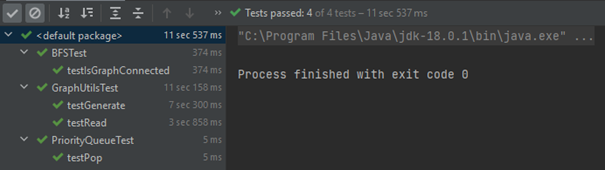
\includegraphics[width=\textwidth]{test_results.png}
    \end{center}

\end{document}